\section{Quantum Gates}

Computers use logic gates that map the functions of boolean logic functions. We have talked about
the AND, OR and NOT logic gates. These gates are used to construct the operational units of a
\say{classical} computer. In contrast, quantum computers need logic gates that adhere to the
laws of Quantum Mechanics - the forementioned \textit{quantum gates}.

There are two kinds of quantum gates:
\begin{enumerate}
    \item single-qubit gates, quantum gates that operate on only one qubit, and
    \item multi-qubit gates, quantum gates that operate on multiple qubits or \textit{quantum registers}.
\end{enumerate}

\subsection{Quantum Registers}

On that note, a \textit{quantum register} is the tensor product of multiple qubits. For example,
if we wanted to store the binary number $101_2=5_{10}$ on a quantum computer, we would need three
qubits $\ket{x}=\ket{1},\ket{y}=\ket{0},\ket{z}=\ket{1}$. By combining them using the tensor operator
we create a quantum register

\begin{equation}
    \ket{\phi}=\ket{x}\otimes\ket{y}\otimes\ket{z}\text{ or }\ket{\phi}=\ket{1}\otimes\ket{0}\otimes\ket{1}
\end{equation}

We can also write a shorthand notation for the quantum register $\ket{\phi}$:

\begin{equation}
    \ket{\phi}=\ket{xyz}\text{ or just }\ket{\phi}=\ket{101}
\end{equation}

where $\ket{\phi}\in\mathbb{H}^3$.

\subsection{Single Qubit Gates}

The Identity gate is a quantum gate that operates on a single qubit and leaves it untransformed.
In matrix notation is represented as:
\begin{equation}
    I = \begin{bmatrix}
        1 & 0 \\
        0 & 1
    \end{bmatrix}
\end{equation}

Let $\ket{\phi} = \phi_0\ket{0} + \phi_1\ket{1}$, the Identity gate will tranform the
single qubit as

\begin{equation}
    I\ket{\phi}=\begin{bmatrix}
        1 & 0\\
        0 & 1
    \end{bmatrix}
    \begin{bmatrix}
        \phi_0\\
        \phi_1
    \end{bmatrix}
    =
    \begin{bmatrix}
        1\cdot\phi_0 + 0\cdot\phi_1\\
        0\cdot\phi_0 + 1\cdot\phi_1
    \end{bmatrix}
    =
    \begin{bmatrix}
        \phi_0\\
        \phi_1
    \end{bmatrix}
    = \ket{\phi}
\end{equation}

The schematic representation of the Identity gate is

\begin{figure}[ht]
    \centering
    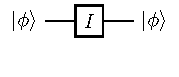
\includegraphics{images/3_Quantum_Computing/identity_gate.pdf}
    \caption{The schematic representation of the Identity gate}
\end{figure}

The NOT gate or $X$ gate is a quantum gate that operates on a single qubit. It tranforms
the qubit by swapping its amplitude coefficients. Let $\ket{\phi} = \phi_0\ket{0} + \phi_1\ket{1}$,
the the $X$ gate will tranform it as

\begin{equation}
    X\ket{\phi}=\begin{bmatrix}
        0 & 1\\
        1 & 0
    \end{bmatrix}
    \begin{bmatrix}
        \phi_0\\
        \phi_1
    \end{bmatrix}
    =
    \begin{bmatrix}
        0\cdot\phi_0 + 1\cdot\phi_1\\
        1\cdot\phi_0 + 0\cdot\phi_1
    \end{bmatrix}
    =
    \begin{bmatrix}
        \phi_1\\
        \phi_0
    \end{bmatrix}
\end{equation}

If the qubit $\ket{\phi}$ was either on state $\ket{0}$ or $\ket{1}$ this gate would
act as a logical negation - flipping the state of the qubit. For example, let
$\ket{\phi} = \ket{0} = 1\cdot\ket{0} + 0\cdot\ket{1}$ then

\begin{equation}
    X\ket{\phi} = 0\cdot\ket{1} + 1\cdot\ket{1} = \ket{1} = \ket{\phi'}
\end{equation}

The schematic representation of the $X$ gate is

\begin{figure}[ht]
    \centering
    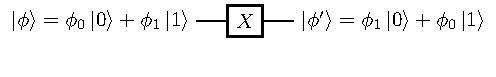
\includegraphics{images/3_Quantum_Computing/x_gate.pdf}
    \caption{The schematic representation of the $X$ gate}
\end{figure}

\begin{figure}[ht]
    \centering
    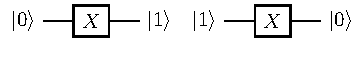
\includegraphics{images/3_Quantum_Computing/x_gate_ex1.pdf}
    \caption{The $X$ gate actions when the input qubit is at the $\ket{0}$ and $\ket{1}$ state respectively}
\end{figure}

The Hadamard gate is a quantum gate that operates on single qubits. It tranforms the qubit by
putting it on a superposition of its basis states. In matrix notation is represented as

\begin{equation}
    H=\frac{1}{\sqrt{2}}\begin{bmatrix}
        1 & 1\\
        1 & -1
    \end{bmatrix}
\end{equation}

Let a single qubit $\ket{\phi}$ have the computation basis $\ket{0},\ket{1}$, then
$\ket{\phi}=\phi_0\ket{0}+\phi_1\ket{1}$. The Hadamard gate will tranform it as

\begin{equation}
    H\ket{\phi}=\frac{1}{\sqrt{2}}\begin{bmatrix}
        1 & 1\\
        1 & -1\\
    \end{bmatrix}
    \begin{bmatrix}
        \phi_0\\
        \phi_1
    \end{bmatrix}
    =\frac{1}{\sqrt{2}}
    \begin{bmatrix}
        1\cdot\phi_0+1\cdot\phi_1\\
        1\cdot\phi_0-1\cdot\phi_1\\
    \end{bmatrix}
    =\frac{1}{\sqrt{2}}[
        (\phi_0+\phi_1)\ket{0}+
        (\phi_0-\phi_1)\ket{1}
    ]
\end{equation}

The schematic representation of the Hadamard gate is

\begin{figure}[ht]
    \centering
    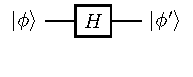
\includegraphics{images/3_Quantum_Computing/hadamard_gate.pdf}
    \caption{The schematic representation of the Hadamard gate}
\end{figure}

We can analyze further by assigning $\ket{\phi}$ to be on the two computation basis states:

\begin{enumerate}
    \item for $\ket{\phi} = \ket{0}$:
    \begin{equation}
        H\ket{\phi}=H\ket{0}=
        H(1\ket{0}+0\ket{1})=
        \frac{1}{\sqrt{2}}[(1+0)\ket{0}+(1-0)\ket{1}]=
        \frac{1}{\sqrt{2}}(\ket{0}+\ket{1})=\ket{+}
    \end{equation}
    \begin{figure}[ht]
        \centering
        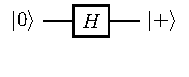
\includegraphics{images/3_Quantum_Computing/hadamard_gate_basis0.pdf}
        \caption{The tranformation of the $\ket{0}$ state to the $\ket{+}$ state}
    \end{figure}
    \item for $\ket{\phi} = \ket{1}$:
    \begin{equation}
        H\ket{\phi}=H\ket{1}=
        H(0\ket{0}+1\ket{1})=
        \frac{1}{\sqrt{2}}[(0+1)\ket{0}+(0-1)\ket{1}]=
        \frac{1}{\sqrt{2}}(\ket{0}-\ket{1})=\ket{-}
    \end{equation}
    \begin{figure}[ht]
        \centering
        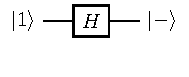
\includegraphics{images/3_Quantum_Computing/hadamard_gate_basis1.pdf}
        \caption{The tranformation of the $\ket{1}$ state to the $\ket{-}$ state}
    \end{figure}
\end{enumerate}

\subsection{Multi-Qubit Gates}

The Controlled-NOT gate or $CX$ gate is a quantum gate that operates on two qubits.
This gate operates by having a \textit{control} and \textit{target} qubit. If
the control qubit is on the $\ket{1}$ state then the target qubit is tranformed
by an $X$ gate tranformation - practically flipping its basis state. In matrix
notation is represented as

\begin{equation}
    CX=\begin{bmatrix}
        1 & 0 & 0 & 0 \\
        0 & 1 & 0 & 0 \\
        0 & 0 & 0 & 1 \\
        0 & 0 & 1 & 0 \\
    \end{bmatrix}
\end{equation}

Let $\ket{\phi}$ be a quantum register of two qubits $\ket{x},\ket{y}$. Then
$\ket{\phi}=\ket{x\otimes y}=\ket{xy}$. We shall note the matrix and linear notation
of the quantum register is

\begin{equation}
    \ket{\phi}=
    \begin{bmatrix}
        x_0y_0\\
        x_0y_1\\
        x_1y_0\\
        x_1y_1
    \end{bmatrix}=
    \begin{bmatrix}
        \phi_0\\
        \phi_1\\
        \phi_2\\
        \phi_3
    \end{bmatrix}=
    \phi_0\ket{00}+\phi_1\ket{01}+\phi_2\ket{10}+\phi_3\ket{11}
\end{equation}

The $CX$ gate will act upon $\ket{\phi}$ as follows

\begin{equation}
    CX\ket{\phi}=\begin{bmatrix}
        1 & 0 & 0 & 0 \\
        0 & 1 & 0 & 0 \\
        0 & 0 & 0 & 1 \\
        0 & 0 & 1 & 0
    \end{bmatrix}
    \begin{bmatrix}
        \phi_0 \\
        \phi_1 \\
        \phi_2 \\
        \phi_3
    \end{bmatrix}=
    \begin{bmatrix}
        \phi_0 \\
        \phi_1 \\
        \phi_3 \\
        \phi_2
    \end{bmatrix}=
    \phi_0\ket{00}+\phi_1\ket{01}+\phi_3\ket{10}+\phi_2\ket{11}
\end{equation}

The schematic representation of the $CX$ gate is
\begin{figure}[ht]
    \centering
    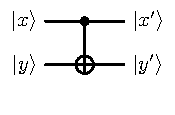
\includegraphics{images/3_Quantum_Computing/cx_gate.pdf}
    \caption{The schematic representation of the $CX$ gate}
\end{figure}

Lastly we will discuss the Controlled-CX gate or $CCX$ gate. The $CCX$ gate is quantum
gate that operates on three qubits. This gate is similar to the $CX$ gate but instead
of having only one control qubit it has two. In matrix notation is represented as

\begin{equation}
    CCX=\begin{bmatrix}
        1 & 0 & 0 & 0 & 0 & 0 & 0 & 0 \\
        0 & 1 & 0 & 0 & 0 & 0 & 0 & 0 \\
        0 & 0 & 1 & 0 & 0 & 0 & 0 & 0 \\
        0 & 0 & 0 & 1 & 0 & 0 & 0 & 0 \\
        0 & 0 & 0 & 0 & 1 & 0 & 0 & 0 \\
        0 & 0 & 0 & 0 & 0 & 1 & 0 & 0 \\
        0 & 0 & 0 & 0 & 0 & 0 & 0 & 1 \\
        0 & 0 & 0 & 0 & 0 & 0 & 1 & 0 \\
    \end{bmatrix}
\end{equation}

Let $\ket{\phi}$ be a quantum register of three qubits $\ket{x},\ket{y},\ket{z}$. Then
$\ket{\phi}=\ket{x\otimes y\otimes z}=\ket{xyz}$. We shall note the matrix and linear notation
of the quantum register is

\begin{equation}
    \ket{\phi}=
    \begin{bmatrix}
        x_0y_0z_0\\
        x_0y_0z_1\\
        x_0y_1z_0\\
        x_0y_1z_1\\
        x_1y_0z_0\\
        x_1y_0z_1\\
        x_1y_1z_0\\
        x_1y_1z_1\\
    \end{bmatrix}=
    \begin{bmatrix}
        \phi_0\\
        \phi_1\\
        \phi_2\\
        \phi_3\\
        \phi_4\\
        \phi_5\\
        \phi_6\\
        \phi_7
    \end{bmatrix}=
    \phi_0\ket{000}+\phi_1\ket{001}+\phi_2\ket{010}+\phi_3\ket{011}+\phi_4\ket{100}+\phi_5\ket{101}+\phi_6\ket{110}+\phi_7\ket{111}
\end{equation}

The $CCX$ gate will act upon $\ket{\phi}$ as follows

\begin{equation}
    CCX\ket{\phi}=\begin{bmatrix}
        1 & 0 & \hdots & 0 & 0 \\
        0 & 1 & \hdots & 0 & 0 \\
        \vdots & \vdots & \ddots & \vdots & \vdots \\
        0 & 0 & \hdots & 0 & 1 \\
        0 & 0 & \hdots & 1 & 0 \\
    \end{bmatrix}
    \begin{bmatrix}
        \phi_0\\
        \phi_1\\
        \vdots \\
        \phi_6\\
        \phi_7
    \end{bmatrix}=
    \begin{bmatrix}
        \phi_0\\
        \phi_1\\
        \vdots \\
        \phi_7\\
        \phi_6
    \end{bmatrix}=
    \phi_0\ket{000}+\phi_1\ket{001}+\hdots+\phi_7\ket{110}+\phi_6\ket{111}
\end{equation}

The schematic representation of the $CCX$ gate is

\begin{figure}[ht]
    \centering
    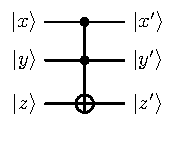
\includegraphics{images/3_Quantum_Computing/ccx_gate.pdf}
    \caption{The schematic representation of the $CCX$ gate}
\end{figure}